\documentclass[a4paper]{article}
\usepackage[spanish,es-tabla]{babel}  %babel es el paquete de idiomas y antes de eso va el o los idiomas que se reuqieren emplear
\usepackage[utf8]{inputenc}
\usepackage{graphicx}
\usepackage{subcaption}
\usepackage[colorlinks=true, citecolor=blue, final]{hyperref}
\usepackage[table]{xcolor}
\usepackage{amsmath}
\usepackage{amssymb}
\setlength{\arrayrulewidth}{1mm}
\setlength{\tabcolsep}{18pt}
\renewcommand{\arraystretch}{2.5}

\usepackage{url} % UTILIZA EL PAQUETE PARA QUE APAREZCA EL URL AUNQUE AUN NOSE SI DEBO ACTIVARLO TAMBIEN EN REFERENCIAS
\hypersetup{
    colorlinks=true,
    linkcolor=blue,
    filecolor=blue,      
    urlcolor=blue,
}
\usepackage{epsfig}
\hypersetup{colorlinks=true,
    linkcolor=blue,
    filecolor=blue,      
    urlcolor=blue,}

\usepackage{graphicx}
\usepackage[sort&compress, numbers]{natbib}
\usepackage{xcolor}
\usepackage{listings}
\usepackage{ragged2e}
\definecolor{codegreen}{rgb}{0,0.6,0}
\definecolor{codegray}{rgb}{0.5,0.5,0.5}
\definecolor{codepurple}{rgb}{0.58,1,0.82}
\definecolor{backcolour}{rgb}{1,1,0.97}
\lstdefinestyle{mystyle}{
    backgroundcolor=\color{backcolour},   
    commentstyle=\color{codegreen},
    keywordstyle=\color{magenta},
    numberstyle=\tiny\color{codegray},
    stringstyle=\color{codepurple},
    basicstyle=\ttfamily\footnotesize,
    breakatwhitespace=false,         
    breaklines=true,                 
    captionpos=b,                    
    keepspaces=true,                 
    numbers=left,                    
    numbersep=5pt,                  
    showspaces=false,                
    showstringspaces=false,
    showtabs=false,                  
    tabsize=2
}
\lstset{style=mystyle}
\usepackage{media9} % for \includemedia AVOID as about to expire
% \usepackage{pdfpc-commands} % for \inlineMovie OK BUT needs own .sty file see below
% \usepackage{xmpmulti} % For \multiinclude OK BUT uses slides in a sequence
\usepackage{multimedia}
\usepackage{animate} % for \animategraphics
\usepackage{eso-pic} % imagen de fondo

\newcommand\imgFondo{%
   \put(0,0){%
      \parbox[b][\paperheight]{\paperwidth}{%
       \vfill
       \centering
       \includegraphics[width=\paperwidth,height=\paperheight,%
       keepaspectratio]{}%
       \vfill
}}}  
\AddToShipoutPictureBG*{\imgFondo}
\begin{document}  %se utiliza para comenzar lo señalado en el parentesis
\begin{center} %begin para comenzar  agregamos centrar para poner en medio
\large \bf Práctica Nº 6   %\large aumenta ligeramente el texto posterior o alarga 
\\ %\\ Indica brincar espacio. \bf indicara subrayar en negritas las letras despues antes de el termino checar que este en minusculas aveces no entra no se porque pasa un espacio antes y despues de agregar
Sistema multiagente
\end{center} %end terminacion de lo señalado en corchetes en este caso el centrado
\textbf{Nombre:}   %\Textbf marca en negritas la frase entre los corchetes
José Adrián García Fuentes
\hfill  %hfill genera un espacio horizontal para expandirse a lo largo del documento
\textbf{Profesor:}   %para que entre el textbf checar que este todo en minusculas
Satu Elisa Schaeffer \hfill
\\
\textbf{Fecha:} 21/Marzo/2021        %\today agrega la fecha en formato de mes dia, año en ingles agregar un usepackage al principio entre llaves el idioma a emplear y entre corchetes babel que es el paquete de idiomas
\\
\hrule    %hrule agrega una linea horizontal en el documento
\medskip
   %bigskip hace espacio grande entre parrafos medskyp tamaño medio y small skyp uno pequeño  si solo pasas espacios no se despega de una linea y marca error
 \section{Introducción}
\justify Un sistema multiagente es un poco como un autómata celular: hay un conjunto de entidades con estados internos que pueden observar estados de los otros y reaccionar cambiando su propio estado. La diferencia es que un sistema multiagente es un concepto más general y permite que estos agentes se muevan y varíen su vecindad, entre otras cosas. En la sexta práctica se implementará un sistema multiagente con una aplicación en epidemiología. Los agentes podrán estar en uno de tres estados: \textbf{s}usceptibles, \textbf{i}nfectados o \textbf{r}ecuperados (esto se conoce como el modelo SIR) \cite{p5}.

\justify Los parámetros serán el número de agentes $n$ y la probabilidad de infección al inicio $P_i$. Vamos a suponer, por simplicidad, que la infección produce inmunidad en los recuperados, por lo cual solamente los susceptibles podrán ser infectados. La probabilidad de contagio será en nuestro caso proporcional a la distancia euclidiana entre dos agentes $d(i,j)$  de la siguiente manera \eqref{eq1}:
\justify
\begin{equation}
$P_c =$\left\{ \begin{array}{b} 0, \qquad si $d(i,j)$\ge $r$, \qquad \qquad \qquad \qquad \qquad  \qquad  \qquad \qquad \qquad \qquad\\\displaystyle{r-d \over r},\qquad $en otro caso$,\qquad \qquad \qquad \qquad \qquad \qquad \qquad \qquad \qquad \qquad 
\end{array}
\label{eq1}
\end{equation}
\medskip
\justify donde $r$ es un umbral \cite{p5}.\justify
Nuestros agentes tendrán coordenadas $x$ y $y$ , una dirección y una velocidad (expresadas las dos últimas simplemente en términos de $\triangle x$ y  $\triangle y$). Vamos a posicionar los agentes, por ahora, uniformemente al azar en un torus formado por doblar un rectángulo de  \textit{l} $x$  \textit{l}, visualizando en todo momento el rectángulo en dos dimensiones \cite{p5}.

\section{Objetivo}  %\section da enfasis a empezar una nueva seccion o tema
\begin{itemize}   %begin comenzar itemize es una viñeta se marca como item no es necesario agregar espacio despues de cada item
 \item Vacunar con probabilidad $P_v$ a los agentes al momento de crearlos de tal forma que están desde el inicio en el estado R y ya no podrán contagiarse ni propagar la infección \cite{p5}.
    \item Estudiar el efecto estadístico del valor de $P_v$ en el porcentaje máximo de infectados durante la simulación y el momento en el cual se alcanza ese máximo \cite{p5}.

\end{itemize}
%\\ Indica brincar espacio.
\section{Metodología}
\justify
La metodología empleada se realizó a través de RStudio \cite{RStudio} llevando a cabo los pasos señalados en la \textit{Práctica 6: Sistema multiagente} \cite{p5}, a partir del código en el repositorio de Schaeffer \cite{p3gitdr}, se hicieron modificaciones para tener un sistema multiagente en el que nuestro agente no viviera en una posición fija en la celda sino que pudiera moverse de posición en el cuadro, cada agente estará en uno de 3 posibles estados (susceptibles, infectados o recuperados) la probabilidad de la infección inicial es $0.05 \%$ y la velocidad máxima es $1/30$  la proporción de recuperación será $0.02 \%$, el código completo de la metodología empleada se encuentra en el repositorio de GitHub \cite{gitadrian}.
\begin{lstlisting}
pi <- 0.05
pr <- 0.02
v <- l / 30
pv <- 0 
pv_paso <- 0.10
for (vac in 1:11) {
  agentes <- data.frame(x = double(), y = double(),
                        dx = double(), dy = double(),
                        estado  = character())
  rnd<-runif(1)
  for (i in 1:n) {
    rnd<-runif(1)
    if (rnd < pv) {
      e <- "R"
    } else {
      e <- "S"
      if (rnd < pi) {
        e <- "I"
      }
    }
    agentes <- rbind(agentes, data.frame(x = runif(1, 0, l),
                                         y = runif(1, 0, l),
                                         dx = runif(1, -v, v),
                                         dy = runif(1, -v, v),
                                         estado = e))
  }
  levels(agentes$estado) <- c("S", "I", "R")
  epidemia <- integer()
  r <- 0.1
  rm <- 0.3
  pm <- 0.2
  ka <- 5
  tmax <- 100
  digitos <- floor(log(tmax, 10)) + 1
  for (tiempo in 1:tmax) {
    infectados <- dim(agentes[agentes$estado == "I",])[1]
    epidemia <- c(epidemia, infectados)
    if (infectados == 0) {
      break
    }
    contagios <- rep(FALSE, n)
    for (i in 1:n) {
      a1 <- agentes[i, ]
      if (a1$estado == "I") {
        for (j in 1:n) {
          if (!contagios[j]) {
            a2 <- agentes[j, ]
            if (a2$estado == "S") {
              dx <- a1$x - a2$x
              dy <- a1$y - a2$y
              d <- sqrt(dx^2 + dy^2)
              if (d < r) {
                p <- (r - d) / r
                if (runif(1) < p) {
                  contagios[j] <- TRUE
                }
              }
            }
          }
        }
      }
    }
    for (i in 1:n) {
      a <- agentes[i, ]
      if (contagios[i]) {
        a$estado <- "I"
      } else if (a$estado == "I") {
        if (runif(1) < pr) {
          a$estado <- "R"
        }
      }
      a$x <- a$x + a$dx
      a$y <- a$y + a$dy
      if (a$x > l) {
        a$x <- a$x - l
      }
      if (a$y > l) {
        a$y <- a$y - l
      }
      if (a$x < 0) {
        a$x <- a$x + l
      }
      if (a$y < 0) {
        a$y <- a$y + l
      }
      agentes[i, ] <- a
    }
    aS <- agentes[agentes$estado == "S",]
    aI <- agentes[agentes$estado == "I",]
    aR <- agentes[agentes$estado == "R",]
    tl <- paste(tiempo, "", sep="")
    while (nchar(tl) < digitos) {
      tl <- paste("0", tl, sep="")
    }
    salida <- paste("p6_t", tl, ".png", sep="")
    tiempo <- paste("Paso", tiempo)
    png(salida)
    plot(l, type="n", main=tiempo, xlim=c(0, l), ylim=c(0, l), xlab="x", ylab="y")
    if (dim(aS)[1] > 0) {
      points(aS$x, aS$y, pch=15, col="chartreuse3", bg="chartreuse3")
    }
    if (dim(aI)[1] > 0) {
      points(aI$x, aI$y, pch=16, col="firebrick2", bg="firebrick2")
    }
    if (dim(aR)[1] > 0) {
      points(aR$x, aR$y, pch=17, col="goldenrod", bg="goldenrod")
    }
    graphics.off()
  }
\end{lstlisting}

\section{Resultados}
\justify
Se obtuvo el código secuencia de GitHub de Schaeffer \cite{p3gitdr} y se añadió probabilidad de vacunación a los agentes al momento de crearlos de tal forma que desde el inicio están en el estado recuperado y ya no podrán contagiarse ni propagar la infección se obtuvo el efecto estadístico del valor de probabilidad de vacunación (cuadro \ref{eq1}) en el porcentaje máximo de infectados durante la simulación y el momento en el cual se alcanza el máximo se generó un archivo .gif \cite{gif} de la simulación en la figura \ref{fig:5} se muestra la posición de los agentes cada uno al momento de iniciar tuvo una probabilidad de vacunación.
\bigskip
\begin{figure}[h!]
    \centering
\begin{subfigure}[b]{0.4\linewidth}
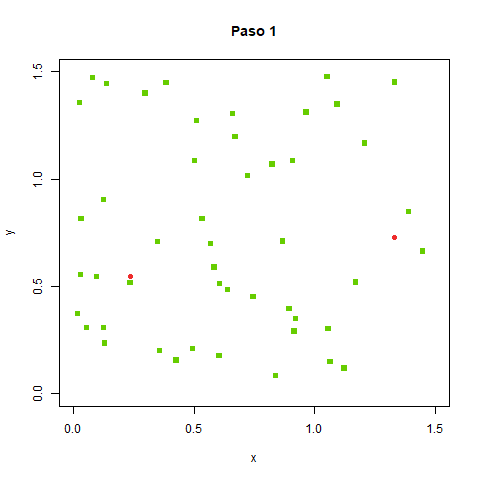
\includegraphics[width=\linewidth]{imagenestareabase/p6_t001.png}
\caption{}
\label{c4}
\end{subfigure}
\begin{subfigure}[b]{0.4\linewidth}
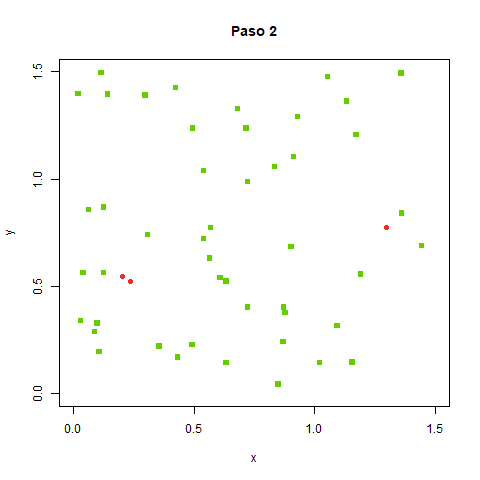
\includegraphics[width=\linewidth]{imagenestareabase/p6_t002.png}
\caption{}
\label{c5}
\end{subfigure}
\caption{Inicio simulación de agentes}
    \label{fig:5}
\end{figure}

\justify Debido a que cada agente ya no propaga la infección y no puede contagiarse al final de la simulación el porcentaje de agentes se encuentra en un estado recuperado para mejor entendimiento ver figura \ref{fig:6}.

\begin{figure}[h!]
    \centering
\begin{subfigure}[b]{0.4\linewidth}
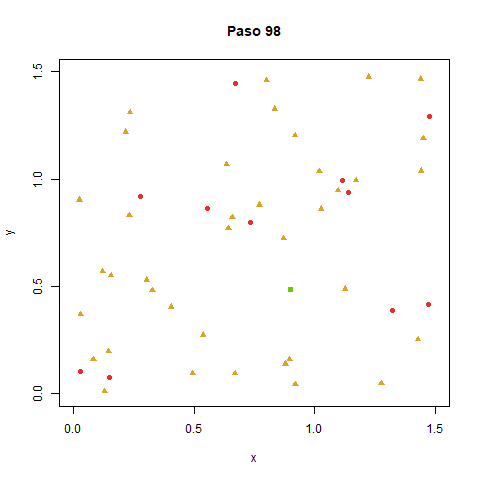
\includegraphics[width=\linewidth]{imagenestareabase/imagenestareabase2/imagenestareabase3/p6_t098.png}
\caption{}
\label{c6}
\end{subfigure}
\begin{subfigure}[b]{0.4\linewidth}
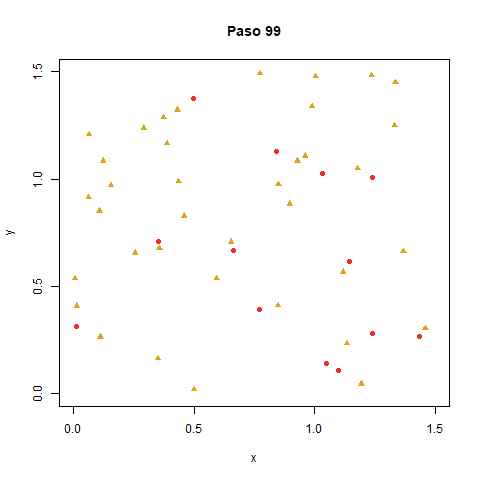
\includegraphics[width=\linewidth]{imagenestareabase/imagenestareabase2/imagenestareabase3/p6_t099.png}
\caption{}
\label{c7}
\end{subfigure}
\caption{Fin de simulación de agentes}
    \label{fig:6}
\end{figure}
\newpage
\justify El efecto estadístico de la probabilidad de vacunación aunque es muy poco variable se observaria que dependiendo de la probabilidad de vacunación existe una ligera disminución en el porcentaje de contagiados salvo algunas exepciones $30 \%$ y $50 \%$.
\justify
\\
\\
\\
\centering
{\rowcolors{3}{blue!90!green!20}{blue!80!yellow!5}
\begin{tabular}{ |p{2.3cm}|p{2cm}|p{2cm}|p{1cm}|}

\hline
\multicolumn{3}{|c|}{Efecto estadístico del valor de probabilidad de vacunación.} \\

\hline
\label{m}
\caption{Efecto estadistico del valor de probabilidad de vacunación.}
Probabilidad de vacunación & Máximo de infectados & Momento máximo de infectados (t) \\
\hline

 \raggedleft$0\%$ & \raggedleft$65\%$ & $49$ \\ 
 \raggedleft$10\%$ & \raggedleft$60\%$ & $52$ \\
 \raggedleft$20\%$ & \raggedleft$58\%$   & $ 19$ y $38$ \\
 \raggedleft$30\%$ & \raggedleft$82\%$ & $17$ \\
 \raggedleft$40\%$ & \raggedleft$56\%$ & $20$ \\
 \raggedleft$50\%$ & \raggedleft$80\%$ & $17$ y $22$ \\
 \raggedleft$60\%$ & \raggedleft$76\%$ & $20$ \\
 \raggedleft$70\%$  & \raggedleft$68\%$ & $30$ \\
 \raggedleft$80\%$ & \raggedleft$53\%$   & $26$ \\
 \raggedleft$90\%$ & \raggedleft$50\%$ & $60$ \\
 \raggedleft$100\%$ & \raggedleft$0\%$ & $0$ \\
 
\hline
\end{tabular}
}


\newpage
\justify Al comparar que la población de agentes se encuentra completamente vacunada (figura \ref{123}) con una vacunación nula (figura \ref{c12}) se observa un porcentaje alto de agentes infectados (ver figura \ref{x})
\begin{figure}[h!]
    \centering
\begin{subfigure}[b]{0.45\linewidth}
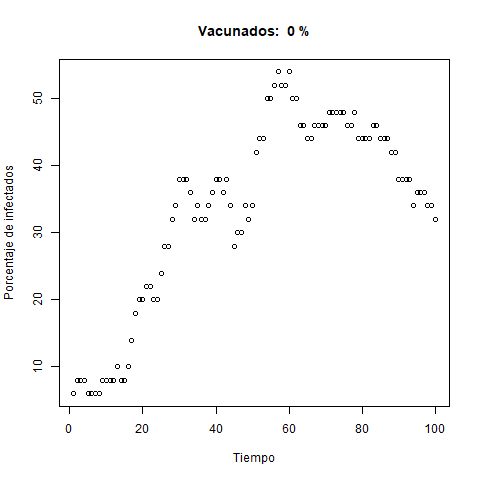
\includegraphics[width=\linewidth]{imagenestareabase/imagenestareabase2/imagenestareabase3/vacuna=0.png}
\caption{}
\label{c12}
\end{subfigure}
\begin{subfigure}[b]{0.45\linewidth}
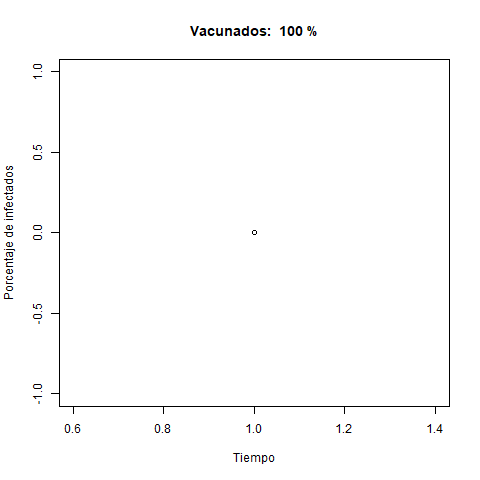
\includegraphics[width=\linewidth]{imagenestareabase/imagenestareabase2/imagenestareabase3/vacuna=1.png}
\caption{}
\label{x}
\end{subfigure}
\caption{Comparación de agentes completamente vacunados con ningun agente vacunado.}
\label{123}
\end{figure}

\justify Aunque se experaría que a mayor porcentaje de vacunados el porcentaje máximo de infectados disminuyera gradualmente existen algunas variantes como ejemplo se muestra la figura \ref{c14} donde una probabilidad del $20 \%$ de agentes vacunados mostró un pico más alto que la probabilidad del $10 \%$ y se observa un repunte en el contagio en los tiempos $19$ y $38$ o bien en la figura \ref{c15} donde ocurre lo mismo sin embargo se observa una baja  en el porcentaje de infectados con respecto al tiempo (figura \ref{fig:8}).
\begin{figure}[h!]
    \centering
\begin{subfigure}[b]{0.45\linewidth}
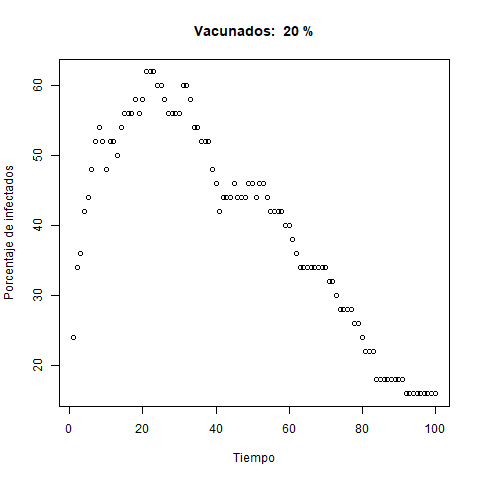
\includegraphics[width=\linewidth]{imagenestareabase/imagenestareabase2/imagenestareabase3/vacuna=0.2.png}
\caption{}
\label{c14}
\end{subfigure}
\begin{subfigure}[b]{0.45\linewidth}
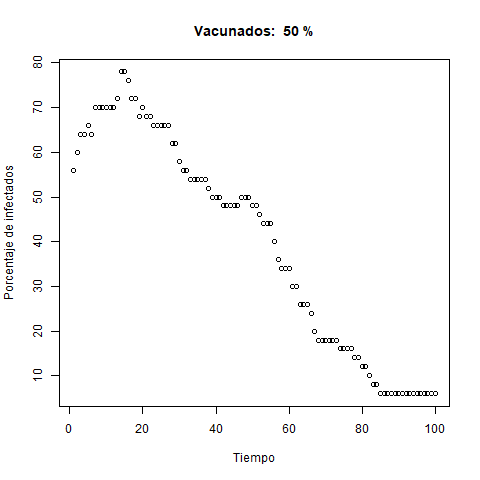
\includegraphics[width=\linewidth]{imagenestareabase/imagenestareabase2/imagenestareabase3/vacuna=0.5.png}
\caption{}
\label{c15}
\end{subfigure}
\caption{Comparación de porcentaje de vacunacion con inconsistencias.}
    \label{fig:8}
\end{figure}

\justify En la figura \ref{fig:15} se encuentra un gráfico de caja-bigote que determina el número de infectados por cada porcentaje de vacunados de manera descendente. 

\begin{figure}[h!]
    \centering
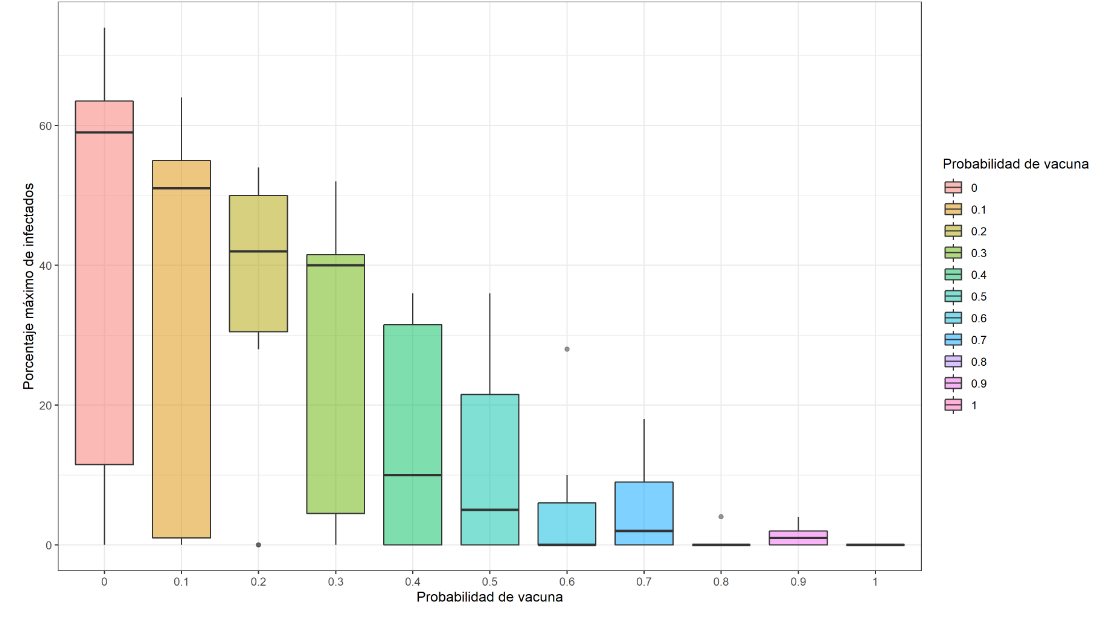
\includegraphics[width=70mm]{porcientos.png}
\caption{Comparación de porcentaje de vacunación}
    \label{fig:15}
\end{figure}
\section{Conclusión}
\justify Al estudiar el efecto estadístico del valor de la probabilidad de vacunación con el porcentaje de agentes infectados en primera instancia se esperaría que el porcentaje de infectados disminuyera de forma gradual hasta que el total de la población de agentes estuviera completamente vacunado sin embargo en dos ocasiones se obtiene inconsistencias que tal vez estén dadas por las direcciones en las que los agentes se desplazan, un ejemplo simple sería la pandemia por Covid-19 en la que  aunque la población no esté vacunada se tienen repuntes de contagios.  


\newpage
\section{Reto 1}
\justify Cambiar los patrones de movimiento para que no tengan una trayectoria fija, cambiar los agentes a que utilize el modelo de punto intermedio aleatorio (inglés: random waypoint model): cada agente tiene una posición meta $(x, y)$  hacia al cual se mueve con una velocidad $v$; al alcanzar (o superar) su meta, elige al azar una nueva meta uniformemente al azar. La velocidad de cada agente es una constante, normalmente distribuido sobre la población de agentes. Examina si surgieron cambios en el efecto de $P_v$ por esta modificación \cite{p5}.

\justify Se obtuvo un código similar de GitHub de Vázquez \cite{gitvazquez} y se adaptó una meta cambiante para cada agente el objetivo es concluir si este nuevo tipo de movimiento de los agentes afecta o no la conclusión anterior.
\begin{lstlisting}
xc<-runif(1,0,1)
yc<-runif(1,0,1)
px<-runif(1,0,1)
py<-runif(1,0,1)
\end{lstlisting}
Al declarar los puntos iniciales en los que aparecen los agentes y sus puntos meta, se genera un número aleatorio de pasos con el que se calcula la velocidad con la que avanza el punto meta cada agente en la figura \ref{reto1} se muestra un diagrama caja-bigote de manera descendente aunque en comparación del gráfico de la tarea base los valores en el porcentaje de infectados no son tan separados se concentran en un rango ligeramente alto.
\begin{lstlisting}
vx<-((px-xc/pasos)
vy<-((py-yc)/pasos)
\end{lstlisting}
\begin{figure}[h!]
    \centering

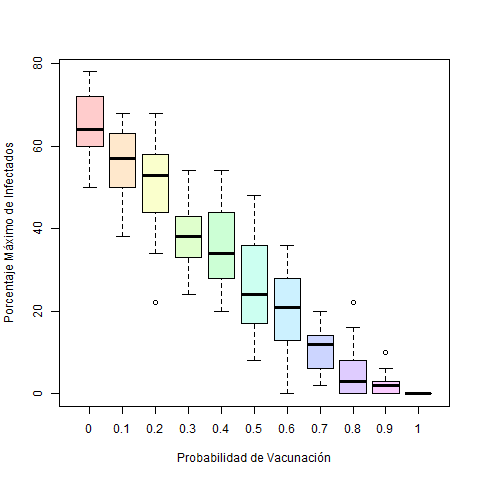
\includegraphics[width=70mm]{reto1 porcentajes.png}
\label{c13}
\caption{Gráfico caja-bigote porcentaje de infectados al establecer un punto meta aleatorio.}
    \label{reto1}
\end{figure}

\section{Conclusión}
 \justify Se obtiene el mismo efecto en el que el valor de $P_v$ afecta el porcentaje de infectados sin embargo debido a que las interacciones entre agentes son muy variables el porcentaje de infectados por tiempo es mayor para cada valor de $P_v$.

\section{Reto 2}
\justify Los agentes tienen amistades: si se encuentran a una distancia euclidiana no mayor a $r_a$ de un amigo suyo, se disminuye su velocidad a la mitad por $k_a$ iteraciones (para saludar a su amigo). Cada par de agentes tiene una amistad con una probabilidad $P_a$. Examina nuevamente si surgieron cambios en el efecto de $P_v$ por esta modificación, con valores $0 < r_a < 1$, $k_a > 1$ y $0 < P_a << 1$ de tu elección \cite{p5}.

\begin{lstlisting}

library(gifski)

setwd("C:/Users/ADRIAN GARCIA/Documents/practica6") 

l <- 1.5
n <- 50
pi <- 0.05
pr <- 0.02
v <- l / 30
pa<-0.02
pv <- 0 
pv_paso <- 0.10

for (vac in 1:11) {
  agentes <- data.frame(x = double(), y = double(),
                        dx = double(), dy = double(),
                        estado  = character())
  rnd<-runif(1)
for (i in 1:n) {
  rnd<-runif(1)
  if (rnd < pv) {#vacunados
    e <- "R"
  } else {
    e <- "S"
    if (rnd < pi) {
      e <- "I"
    }
  }
  agentes <- rbind(agentes, data.frame(x = runif(1, 0, l),
                                       y = runif(1, 0, l),
                                       dx = runif(1, -v, v),
                                       dy = runif(1, -v, v),
                                       estado = e))
}

levels(agentes$estado) <- c("S", "I", "R")
epidemia <- integer()
r <- 0.1
rm <- 0.3
pm <- 0.2
ka <- 5
tmax <- 100
digitos <- floor(log(tmax, 10)) + 1

for (tiempo in 1:tmax) {
  infectados <- dim(agentes[agentes$estado == "I",])[1]
  epidemia <- c(epidemia, infectados)
  if (infectados == 0) {
    break
  }
  contagios <- rep(FALSE, n)
  for (i in 1:n) { 
    a1 <- agentes[i, ]
    if (a1$estado == "I") { 
      for (j in 1:n) {
        if (!contagios[j]) {
          a2 <- agentes[j, ]
          if (a2$estado == "S") {
            dx <- a1$x - a2$x
            dy <- a1$y - a2$y
            d <- sqrt(dx^2 + dy^2)
            if (d < rm) { # umbral amistad
              p <- (r - d) / r
              if (runif(1) < pm) {
                for (i in 1:ka) { 
                dx <- (a1$x - a2$x)/2
                dy <- (a1$y - a2$y)/2
                }
              }
            }
            if (d < r) {
              p <- (r - d) / r
              if (runif(1) < p) {
                contagios[j] <- TRUE
              }
            }
          }
        }
      }
    }
  }
  for (i in 1:n) { 
    a <- agentes[i, ]
    if (contagios[i]) {
      a$estado <- "I"
    } else if (a$estado == "I") { 
      if (runif(1) < pr) {
        a$estado <- "R" 
      }
    }
    a$x <- a$x + a$dx
    a$y <- a$y + a$dy
    if (a$x > l) {
      a$x <- a$x - l
    }
    if (a$y > l) {
      a$y <- a$y - l
    }
    if (a$x < 0) {
      a$x <- a$x + l
    }
    if (a$y < 0) {
      a$y <- a$y + l
    }
    agentes[i, ] <- a
  }
  aS <- agentes[agentes$estado == "S",]
  aI <- agentes[agentes$estado == "I",]
  aR <- agentes[agentes$estado == "R",]
  tl <- paste(tiempo, "", sep="")
  while (nchar(tl) < digitos) {
    tl <- paste("0", tl, sep="")
  }
  salida <- paste("p6_t", tl, ".png", sep="")
  tiempo <- paste("Paso", tiempo)
  png(salida)
  plot(l, type="n", main=tiempo, xlim=c(0, l), ylim=c(0, l), xlab="x", ylab="y")
  if (dim(aS)[1] > 0) {
    points(aS$x, aS$y, pch=15, col="chartreuse3", bg="chartreuse3")
  }
  if (dim(aI)[1] > 0) {
    points(aI$x, aI$y, pch=16, col="firebrick2", bg="firebrick2")
  }
  if (dim(aR)[1] > 0) {
    points(aR$x, aR$y, pch=17, col="goldenrod", bg="goldenrod")
  }
  graphics.off()
}
salida <- paste("vacuna=", pv, ".png", sep="")
png(salida)
plot(1:length(epidemia), 100 * epidemia / n, xlab="Tiempo", ylab="Porcentaje de infectados",
  main=paste("Vacunados: ",pv * 100, "%"))
graphics.off()
pv <- pv + pv_paso
}
png_files <- list.files( pattern = "p6_t.*png$", full.names = TRUE)
gifski(png_files, gif_file = "animation.gif", width = 800, height = 600, delay = 1)
\end{lstlisting}
\justify
A partir del código de la tarea base se añadió a cada agente amistades con ($P_a$ de $0.02\%$) y si estos se encontraban a una distancia euclideana de un amigo suyo este disminuiría su velocidad se añadió probabilidad de vacunación a los agentes al momento de crearlos, se obtuvo el efecto estadístico del valor de probabilidad de vacunación (cuadro \ref{fig:6}) en el porcentaje máximo de infectados durante la simulación y el momento en el cual se alcanza el máximo se generó un archivo .gif \cite{gif} de la simulación.
\justify En la figura \ref{qw} se muestran los primeros 4 pasos de una simulación si observamos en el paso uno (\ref{q4}) se encuentra un agente contagiado en la parte central, un poco en la parte superior derecha, en el paso 2 (\ref{q5}) se encuentra con un amigo provocando disminución en su velocidad a la mitad, en el paso 3 (\ref{q6}) se observa que el mismo agente no se separó mucho en distancia del agente con el que se encontró en comparación del movimiento de los otros agentes, observe el paso 4 (\ref{q7}) la distancia entre todos los agentes es mayor en comparación con el agente antes mencionado.
\bigskip
\begin{figure}[h!]
    \centering
\begin{subfigure}[b]{0.45\linewidth}
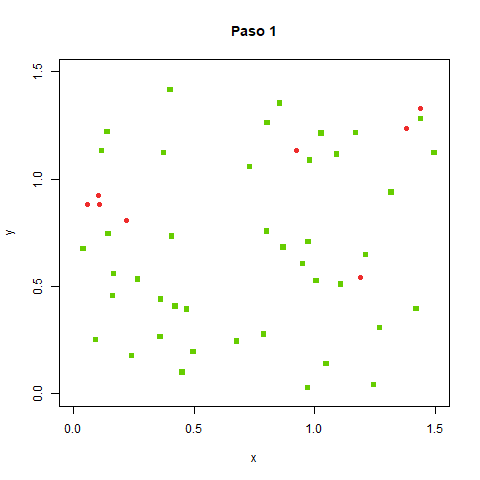
\includegraphics[width=\linewidth]{reto2,1.png}
\caption{}
\label{q4}
\end{subfigure}
\begin{subfigure}[b]{0.45\linewidth}
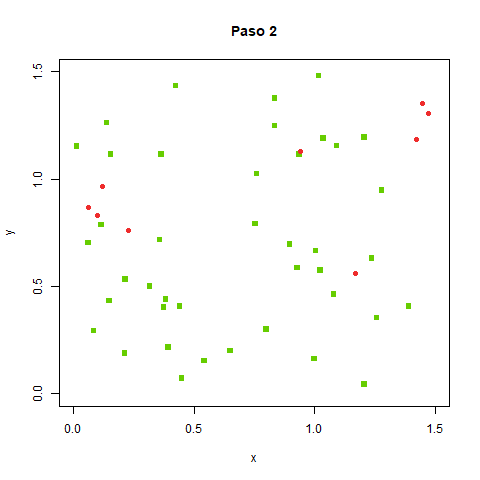
\includegraphics[width=\linewidth]{reto2,2.png}
\caption{}
\label{q5}
\end{subfigure}
\begin{subfigure}[b]{0.45\linewidth}
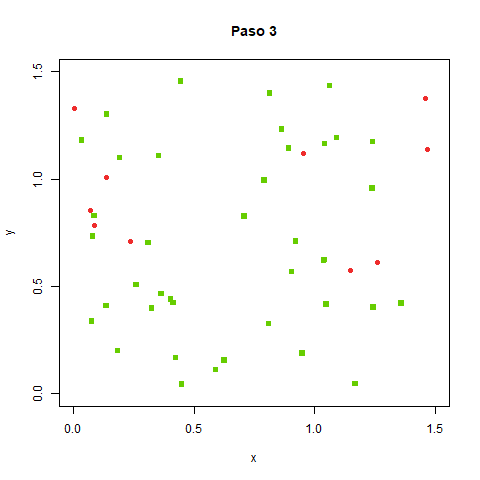
\includegraphics[width=\linewidth]{reto2,3.png}
\caption{}
\label{q6}
\end{subfigure}
\begin{subfigure}[b]{0.45\linewidth}
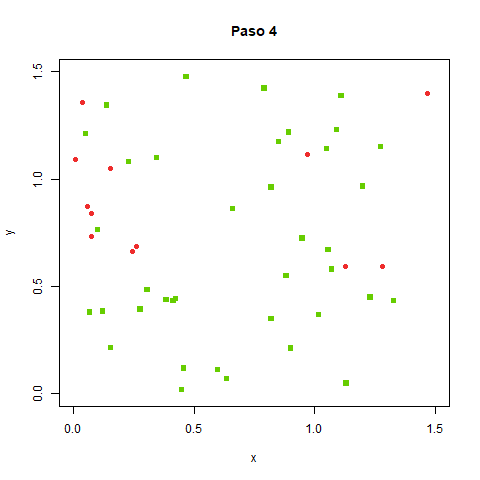
\includegraphics[width=\linewidth]{reto2,4.png}
\caption{}
\label{q7}
\end{subfigure}
\caption{Inicio simulación de agentes}
    \label{qw}
\end{figure}

\justify
\\
\\
\\
\clearpage
\centering
{\rowcolors{3}{red!20!white!40}{red!10!white!20}
\begin{tabular}{ |p{2.3cm}|p{2cm}|p{2cm}|p{1cm}|}

\hline
\multicolumn{3}{|c|}{Efecto estadístico del valor de probabilidad de vacunación.} \\

\hline
\label{m}
\caption{Efecto estadistico del valor de probabilidad de vacunación.}
Probabilidad de vacunación & Máximo de infectados & Momento máximo de infectados (t) \\
\hline

 \raggedleft $0\%$ & \raggedleft $55\%$ &  $60$ \\ 
 \raggedleft $10\%$ & \raggedleft $50\%$ &  $60$ \\
 \raggedleft $20\%$ & \raggedleft $65\%$   &  $30$ \\
 \raggedleft $30\%$ & \raggedleft $56\%$ &  $60$ \\
 \raggedleft $40\%$ & \raggedleft $86\%$ &  $17$ \\
 \raggedleft $50\%$ & \raggedleft $78\%$ &  $22$ \\
 \raggedleft $60\%$ & \raggedleft $78\%$ &  $17$ y $30$ \\
 \raggedleft $70\%$  & \raggedleft $70\%$ &  $18$ \\
 \raggedleft $80\%$  & \raggedleft $82\%$   &  $17$ \\
 \raggedleft $90\%$ & \raggedleft $2\%$ &  $3$ \\
 \raggedleft $100\%$ & \raggedleft $0\%$ &  $0$ \\
 
\hline
\end{tabular}
}


\newpage
\justify Al realizar una comparación con el grafico de la tarea base (figura \ref{q12}) y  el efecto que tiene la probabilidad de amistad (figura \ref{q13}) en los agentes que no se encuentran vacunados (figura \ref{qwer}) se observa un porcentaje alto de agentes infectados (ver figura \ref{qwer}).
\begin{figure}[h!]
    \centering
\begin{subfigure}[b]{0.45\linewidth}
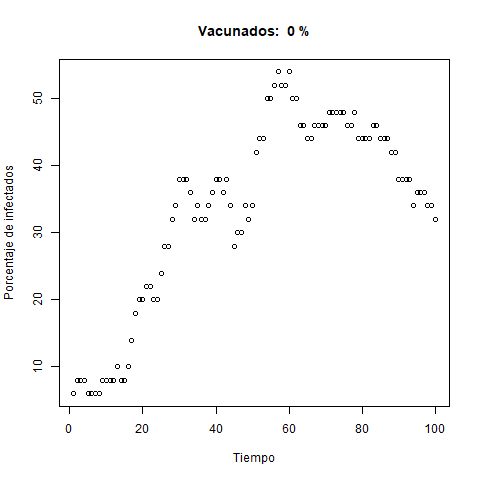
\includegraphics[width=\linewidth]{imagenestareabase/imagenestareabase2/imagenestareabase3/vacuna=0.png}
\caption{}
\label{q12}
\end{subfigure}
\begin{subfigure}[b]{0.45\linewidth}
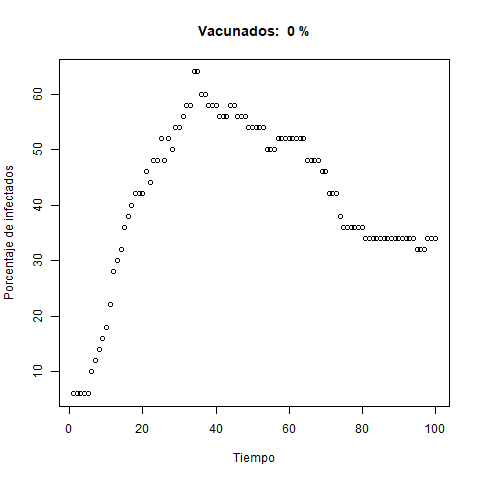
\includegraphics[width=\linewidth]{vacuna reto2.png}
\caption{}
\label{q13}
\end{subfigure}
\caption{Comparación de gráficos tarea base y reto 2.}
    \label{qwer}
\end{figure}

\justify Se obtienen gráficos muy similares  sin embargo el porcentaje de infectados por tiempo es ligeramente mayor tal vez esto sea dado por el tiempo en que se desplazan los agentes cuando interactúan con un amigo y las probabilidades en que otro agente se pueda contagiar dependerán de sí se topan con él.

\section{Conclusión.}
\justify El efecto estadístico de la probabilidad de vacunación en comparación de la tarea base cambia aunque en algunas ocasiones cambia muy poco se podría decir que se mantiene en un porcentaje de infectados en un rango de $55$ a $80$ \% a  excepción del $90$ $\%$ de vacunados que solo se infectó un $2$ $\% $y el tiempo de contagio fue rapido tal vez estos cambios en la variacion de infectados es debido al tiempo en el que se retrasan los agentes al estar con un amigo y acorta de cierta manera la probabilidad de contagio.  

\newpage
\bibliography{practica6} %\bibliography dentro de los corchetes aparece el comando seccion de referencias  sin embargo para que aparezca tiene que aparecer la seccion \bibliographystyle para dar un estilo del tipo de letra o tipo de acomodo que llevara 
\bibliographystyle{ieeetr}   %\da un estilo de acomodo dependiendo del comando dentro d corchetes
\end{document} %indica finalizacion de lo señalado en el parentesis en este caso el documento


